\documentclass[papersize={24in,36in}]{beamer}
\mode<presentation>{\usetheme{src}}
\usepackage{wrapfig}
\usepackage{physics}
\usepackage[style=numeric,backend=biber]{biblatex}
\addbibresource{src_poster.bib}
\usepackage[orientation=portrait,scale=1.4]{beamerposter}
\renewcommand*{\bibfont}{\normalfont\footnotesize}
\graphicspath{{images/}}
\setlogo{images/uvm_logo_white.png}
\title{\huge Precise Control of Organic LED Emission Through Optical Resonance Cavity Encapsulation}
\author{ \textbf{Benjamin Isenhart}\inst{1}, Matthew White\inst{1,2}, Ekraj Dahal\inst{2}, Karen Cianciulli\inst{3}}
\institute[UVM]{\small \inst{1} Department of Physics, the University of Vermont, Burlington VT,\\ \inst{2} Materials Science Program, the University of Vermont, Burlington VT,\\ \inst{3} Asheville School, Asheville NC\\\ }
\date[Apr. 17th, 2019]{Apr. 17th, 2019}

\newlength{\columnheight}
\setlength{\columnheight}{105cm}

\begin{document}
\begin{frame}
  \begin{columns}
    \begin{column}{.49\textwidth}
      \begin{beamercolorbox}[center,wd=\textwidth]{postercolumn}
        \begin{minipage}[T]{.95\textwidth}
			\parbox[t][\columnheight]{\textwidth}{
			\vspace{2cm}
            \begin{block}{Introduction}
				Light emitting diodes (LEDs) have become an integral part of daily life, from televisions to headlights on cars. While LEDs have substantial benefits over incandescent bulbs, they have significant environmental impacts, often using hazardous materials \cite{Lim2011}. This has been mitigated in part by the advent of organic LEDS (OLEDs), which are generally less harmful and expensive, but the emission spectrum of organic molecules is strongly dependent on structure, and thus more difficult to control \cite{Geffroy2006}. In this project, we demonstrate a technique for taking a single organic emitter, and modifying its emission spectrum through device design alone. Additionally, we explore the ability to generate multi-peaked emission profiles with only a single organic emitter material.
            \end{block}
            \vfill
            \begin{block}{Device Fabrication and Characterization}
					\begin{wrapfigure}{r}{0.52\textwidth}
						\centering
						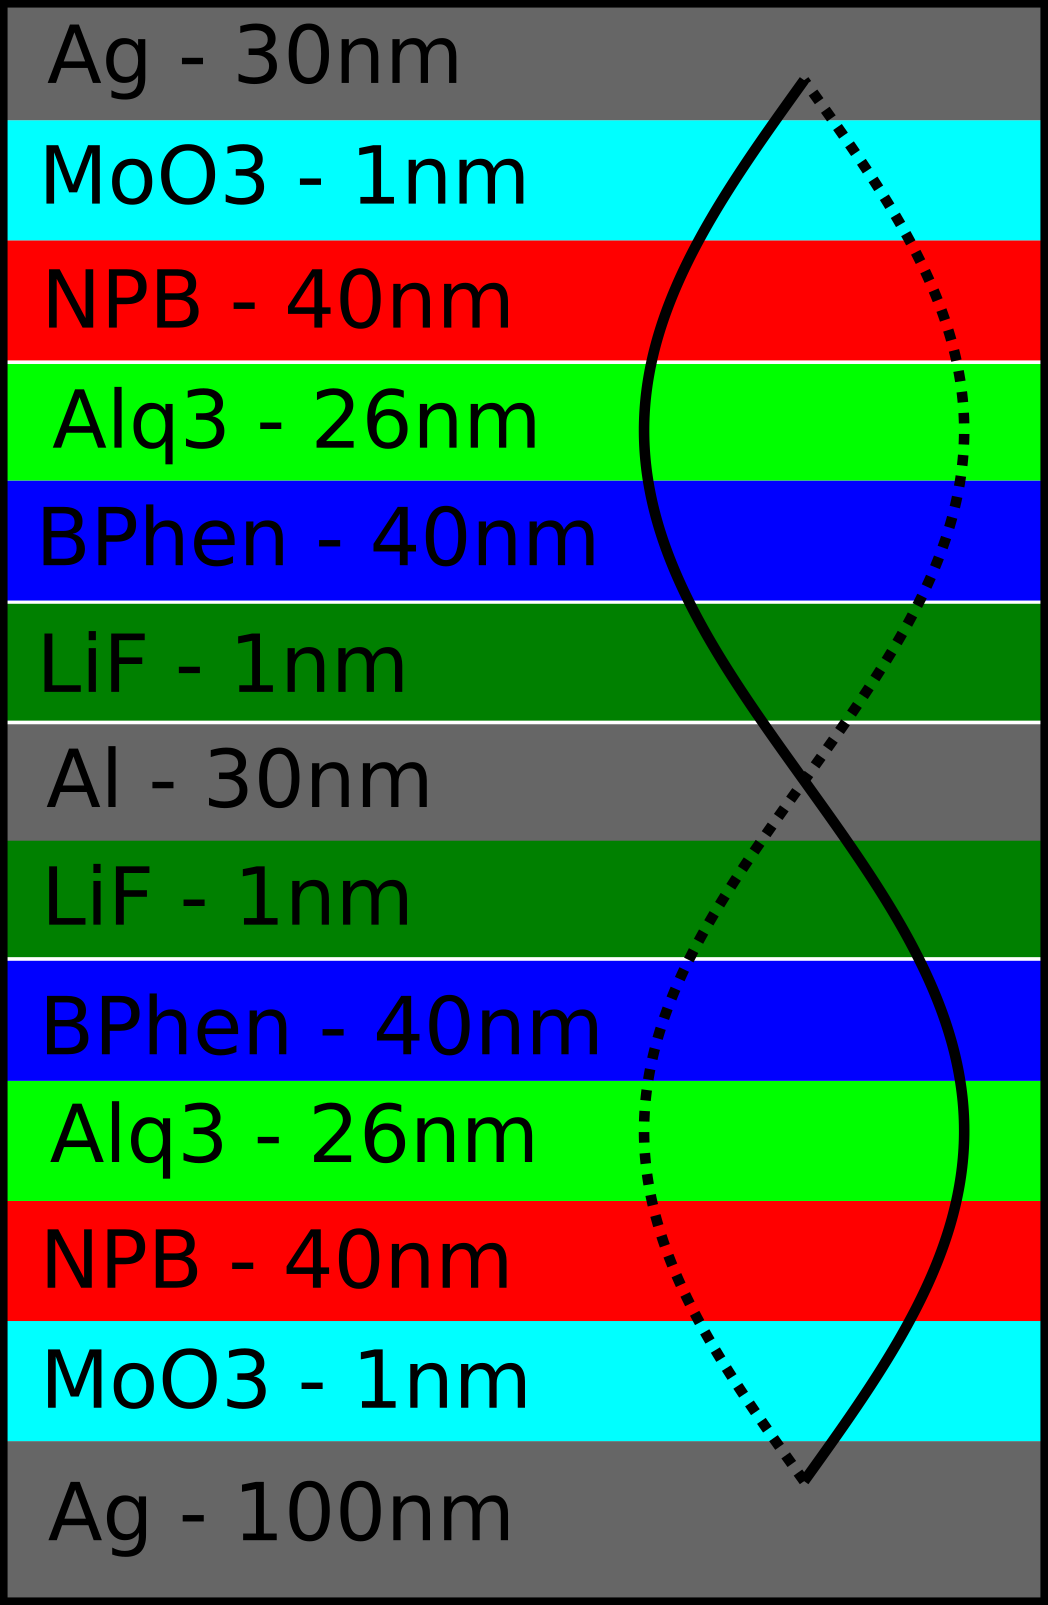
\includegraphics[width=0.3\textwidth]{images/schematic.png}
						\caption{Schematic for a multi-cavity device\newline with half wavelength resonance mode}
					\end{wrapfigure}
					Devices were fabricated through sequential physical vapor deposition under high vacuum. In each device, the bottom electrode was deposited at a thickness of 100nm, while all subsequent electrodes were made at a thickness of 30nm. The organics layer was formed from 40nm/26nm/40nm of NPB/Alq$_3$/BPhen for multi-cavity devices and varying thicknesses in the single cavity devices. Single cavity devices were characterized using forward emission spectroscopy, while multi-cavity devices were characterized using angular resolved spectroscopy, with emission spectra collected at 2.5$^o$ intervals, from 0 to 70$^o$.
            \end{block}
			\vfill
            \begin{block}{Results of Forward Emission Spectroscopy}
			 	In the forward emission of the single cavity devices, we find that the peak emission wavelength can be controlled by varying the thickness of the organics layer, effectively changing the width of the resonance cavity. We find a linear relationship between the peak wavelength and the cavity width 
				\begin{wrapfigure}{r}{0.5\textwidth}
					%\centering
					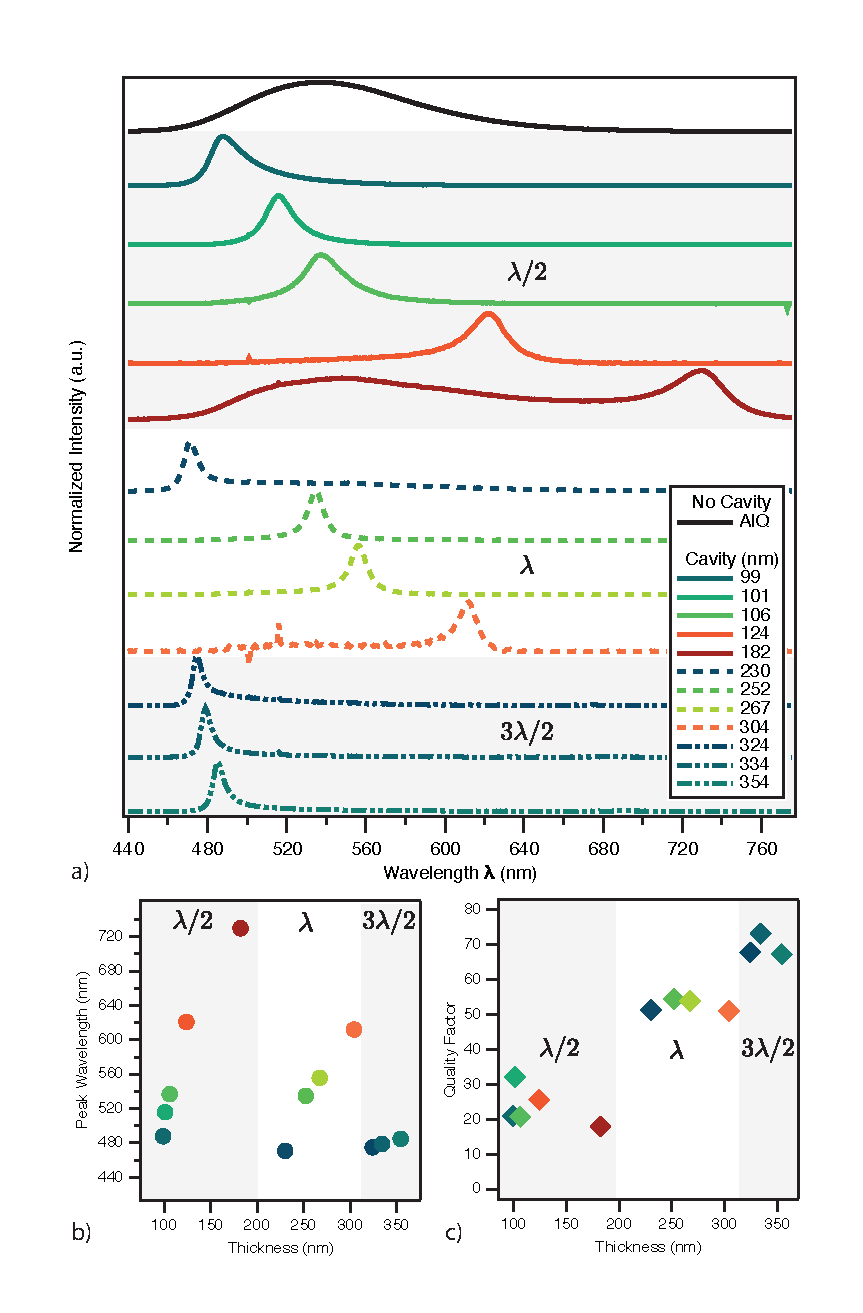
\includegraphics[width=0.45\textwidth]{images/F_N1FPPrelim.pdf}
					\caption{Emission characteristics of single\newline cavity devices:\newline (a): Emission spectrum as a function\newline of cavity thickness,\newline (b): Peak wavelength as a function of \newline cavity thickness,\newline (c): Quality factor as a function of cavity thickness}
				\end{wrapfigure}
				except at transition points where the resonance shifts from an $\frac{n\lambda}{2}$ to an $\frac{\qty(n+1)\lambda}{2}$ resonance. We can also note that the quality factor shows a linear relationship with the cavity thickness. This is congruous with the Heisenberg uncertainty principle in that a thicker resonance cavity increases the uncertainty in the position of the photon, leading to the ability to measure its momentum more precisely. In both cases, we see a strong outlier in the 182nm cavity. However, looking at the spectrum of the 182nm cavity device, we find can see that the resonant mode is accompanied by the broadband emission of Alq$_3$. This is due to the fact that the resonant mode occurs at a wavelength where a very small fraction of the broadband emission is present. Thus, the resonant mode is very dim, and is on a similar order to that of the broadband leakage out of the cavity.
            \end{block}
			\vspace{2cm}
          }
        \end{minipage}
      \end{beamercolorbox}
    \end{column}
    \begin{column}{.49\textwidth}
      \begin{beamercolorbox}[center,wd=\textwidth]{postercolumn}
        \begin{minipage}[T]{.95\textwidth} % tweaks the width, makes a new \textwidth
          \parbox[t][\columnheight]{\textwidth}{
			\vspace{2cm}
            \begin{block}{Results of Angular Resolved Emission Spectroscopy}
				In the angular resolved emission of the single cavity devices, we can notice a mode splitting event at approximately 45$^o$. This, along with the blueshifting at higher angles, is as predicted by basic propagation in a waveguide \cite{Stavrinou1999}. We also notice that there are significant differences between the emission spectra of the two single cavity devices that are inverted with respect
				\begin{wrapfigure}{r}{0.5\textwidth}
					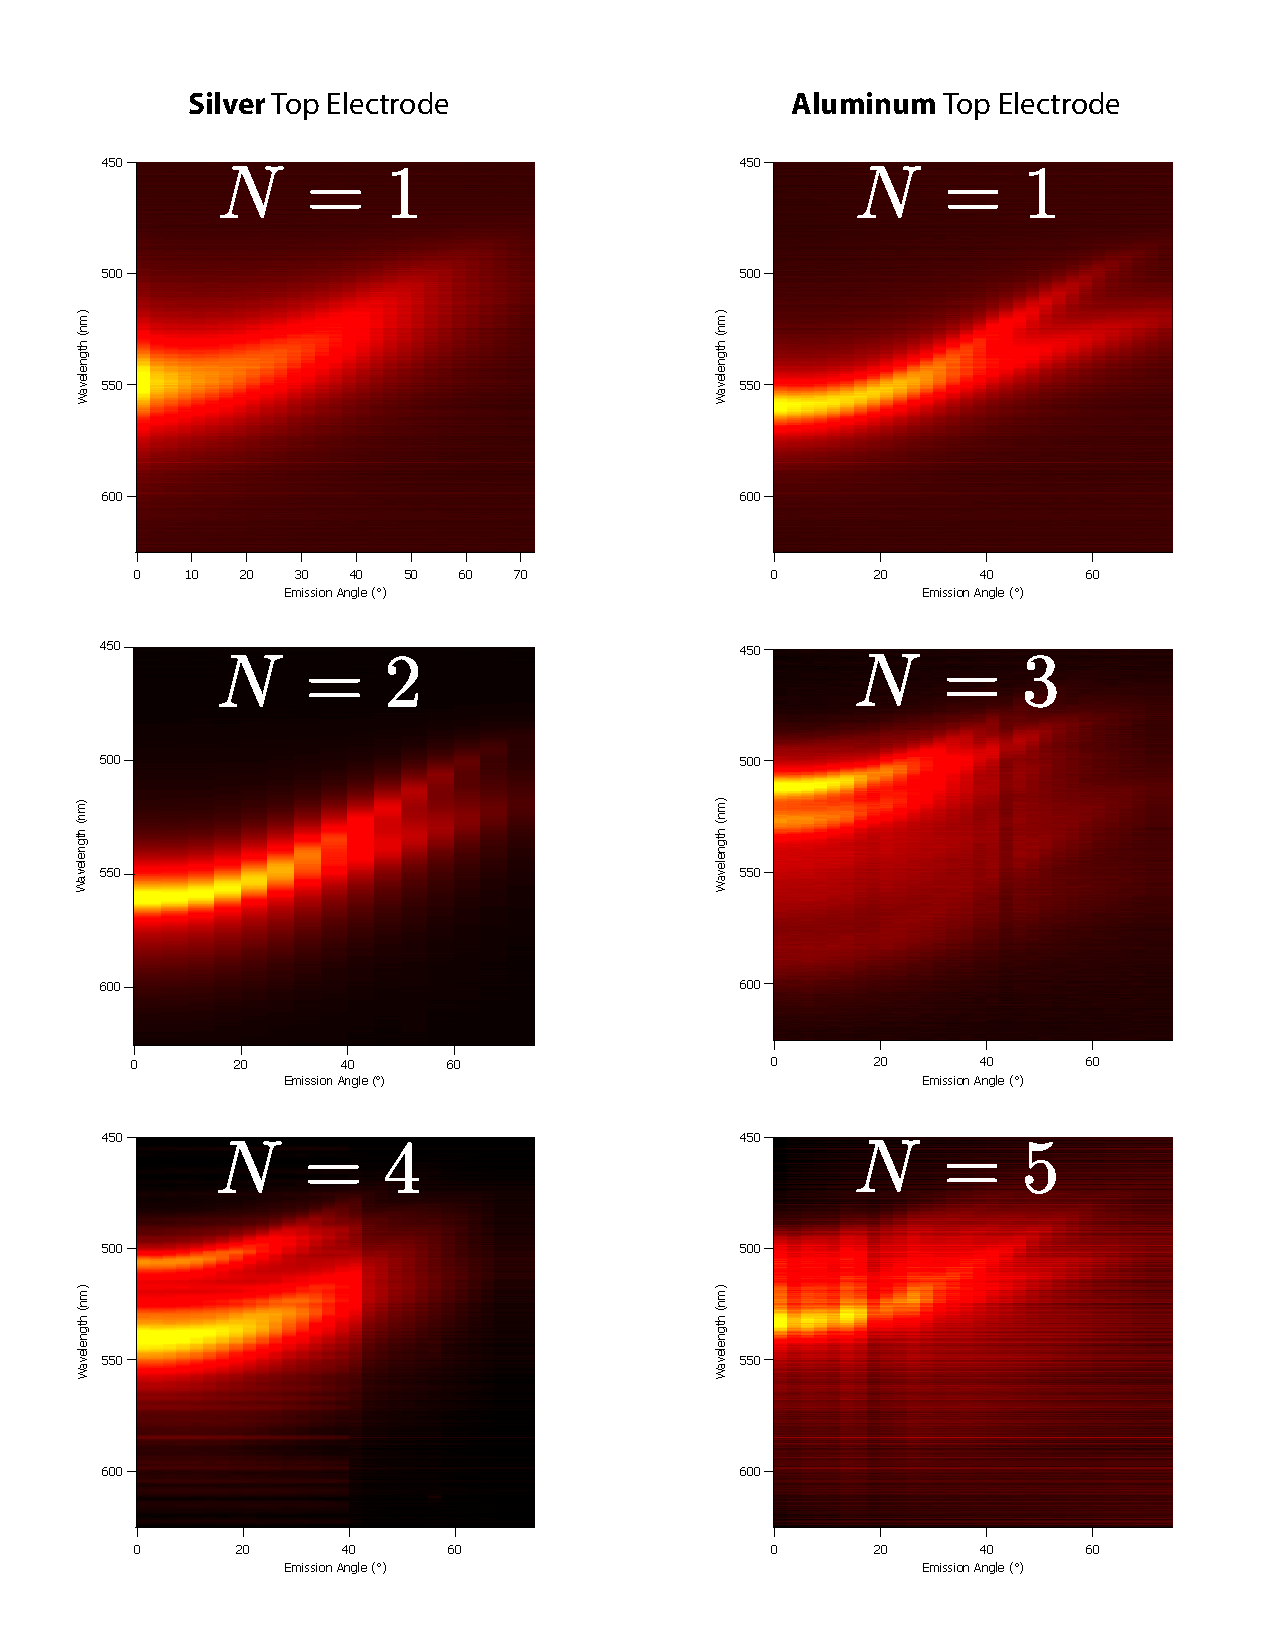
\includegraphics[width=0.4\textwidth]{images/DFDG_Summary.pdf}
					\caption{ Angular resolved emission\newline profiles for resonant microcavity devices}
				\end{wrapfigure}
				to each other. In particular, the emission from the device with a 30nm Al top electrode is narrower and redshifted from the peak of the inverted device, whose peak lies at the peak emission of non-resonant Alq$_3$. This is due to the higher absorption and lower reflectivity of aluminum \cite{Schulz1954}. In the aluminum topped device, there is a 100nm silver back electrode, meaning that any photons traveling toward the back electrode would be strongly reflected at the resonant mode, which can then be transmitted through the 30nm top electrode. Conversely, the silver topped device does not have that strong boundary condition, leading to a larger broadband emission. For devices with multiple cavities, we find a more complex modal structure, even in the forward emission. In the three and four cavity devices, we see two distinct forward emission peaks between 500 and 550nm, and in the five cavity device, we see three distinct emission peaks in the same region. All of these peaks blueshift at higher angles, as would be expected for resonant modes. It can also be seen that the emission spectrum narrows with each additional cavity. This can be explained by the fact that with each additional cavity we obtain another point at which we know the resonant mode must have a node, which gives us a higher certainty in the wavelength of the resonant mode.

            \end{block}
            \vfill
            \begin{block}{Conclusions and Future Works}
				In this project, we have demonstrated a technique to precisely control the peak emission wavelength of an organic LED as well as a method for generating more complex emission profiles. The linearity between cavity thickness and peak emission allows for very exact prediction of emission wavelength for a device, to within the resolution of our ability to deposit films. The modal structure of the multi-cavity devices provide several avenues of potential future exploration, including dependence of modal separation on cavity thickness, behavior at higher numbers of cavities, and structure under higher current densities. A strong understanding of these modal structures could lead to fabrication of devices to match any desired emission spectrum, which could be used to make high quality OLED screens and potentially organic diode lasers.
			\end{block}
			\vfill
			\begin{block}{Acknowledgements}
				We would like to thank the University of Vermont Office of Undergraduate Research and Clean Energy Fund for funding for work on this project during the summer of 2019 and the University of Vermont Department of Physics Crowell Award for funding for the summer of 2018. We would also like to thank the UVM Honors College.
            \end{block}
            \begin{block}{References}
				\printbibliography
			\end{block}
			\vspace{2cm}
          }
        \end{minipage}
      \end{beamercolorbox}
    \end{column}
  \end{columns}
  \vskip1ex
\end{frame}
\end{document}
